\documentclass[11pt,a4paper]{article}
\usepackage[utf8]{inputenc}
\usepackage[T1]{fontenc}
\usepackage{lmodern}
\usepackage[margin=2.3cm]{geometry}
\usepackage{amsmath,amssymb}
\usepackage{graphicx}
\usepackage{booktabs}
\usepackage{multirow}
\usepackage{float}
\usepackage[font=small,labelfont=bf]{caption}
\usepackage{subcaption}
\usepackage{xcolor}
\usepackage{microtype}
\usepackage{tikz}
\usetikzlibrary{positioning,arrows.meta,fit}
\usepackage[colorlinks=true,linkcolor=blue!50!black,citecolor=blue!50!black,urlcolor=blue!50!black]{hyperref}
\graphicspath{{figs/}}
\setlength{\parskip}{0.45em}
\setlength{\parindent}{0pt}
\newcommand{\uhat}{\hat{u}}
\newcommand{\gapv}{\Delta}
\newcommand{\pos}[1]{\textcolor{green!45!black}{#1}}
\newcommand{\negc}[1]{\textcolor{red!65!black}{#1}}

\title{\textbf{Does Closing the Modality Gap Help\\Hard-Negative-Trained CLIP?}\\[0.4em]
\large CS 725 Course Project: Final Report}
\author{Viren Mehta (25M2132) \and Lavanay Thakral (25D0381) \and Shrey Patel (26M1104) \and Yash Chopra (26M1520)}
\date{November 2026}

\begin{document}
\maketitle

\begin{abstract}
CLIP places image and text embeddings in two separate regions of its shared space, the
\emph{modality gap}. Recent work reports that closing this gap after training makes CLIP more robust
without hurting accuracy. NegCLIP-style fine-tuning with hard negative captions and images makes CLIP
compositional. We ask whether the two combine: \textbf{does closing the gap help hard-negative-trained
CLIP?} We fine-tuned CLIP ViT-B/32 on COCO in five configurations (plain, batch-512 plain, + hard
captions, + hard images, and the full NegCLIP recipe) at three learning rates and three seeds (30 runs),
measured the gap, shifted embeddings post hoc in four ways, and evaluated every setting on COCO
retrieval, ARO (COCO-Order, VG-Relation, VG-Attribution) and SugarCrepe, clean and under embedding
noise.

The answer is \textbf{no}. Closing the gap lowers COCO-Order accuracy by 0.21--0.34 and VG-Attribution by
0.04--0.06 for every model trained with hard captions, and lowers retrieval Recall@1 by 0.13--0.20 for
every model. We trace the effect to one mechanism: a shift without re-normalisation changes no ranking,
and the re-normalised shift acts like deleting each caption's own coordinate along the gap direction.
Removing only that coordinate reproduces the full damage (released NegCLIP COCO-Order: $-0.327$ in both
cases). That direction holds under 1\% of the text variance, yet in hard-caption models it carries
word-order and attribute information. During training, hard negative \emph{images} shrink the gap
(0.65 vs 0.78 at lr $5\times10^{-6}$), a batch-size control rules out the larger batch as the cause,
and hard negative \emph{captions} alone give the best compositional scores at every learning rate,
ahead of the released NegCLIP. Gap size and compositional skill are therefore driven by different
ingredients.
\end{abstract}

\tableofcontents
\newpage

%=====================================================================
\section{Introduction}

\paragraph{CLIP and contrastive learning.}
CLIP \cite{clip} trains an image encoder $f$ and a text encoder $g$ so that matching image--caption
pairs have high cosine similarity and mismatched pairs low similarity. Both encoders output
$L_2$-normalised 512-dimensional vectors $x=f(I)$ and $y=g(T)$. For a batch of $N$ pairs, the loss is
a symmetric cross-entropy over the $N\times N$ similarity matrix scaled by a learned temperature $\tau$:
\begin{equation}
\mathcal{L}_{\text{CLIP}}=\frac{1}{2N}\sum_{i=1}^{N}\left[-\log\frac{e^{x_i^\top y_i/\tau}}{\sum_j e^{x_i^\top y_j/\tau}}
-\log\frac{e^{x_i^\top y_i/\tau}}{\sum_j e^{x_j^\top y_i/\tau}}\right].
\end{equation}
This is the InfoNCE objective \cite{infonce} applied across two modalities; Wang and Isola \cite{wangisola}
show it trades off \emph{alignment} of positive pairs and \emph{uniformity} on the sphere.

\paragraph{The modality gap.}
Liang et al.\ \cite{liang} found that CLIP's image and text embeddings occupy two separate, narrow cones.
They measure the gap as the distance between the two centroids,
\begin{equation}
\gapv=\frac{1}{n}\sum_{i=1}^{n}x_i-\frac{1}{n}\sum_{i=1}^{n}y_i,\qquad \text{gap}=\lVert\gapv\rVert_2 ,
\end{equation}
which is about 0.82 for CLIP ViT-B/32 on COCO. Chowers et al.\ \cite{chowers} argue that the gap behaves
like a global vector nearly orthogonal to how embeddings vary, and that closing it post hoc improves
robustness to perturbations without changing clean accuracy.

\paragraph{Bag-of-words behaviour and NegCLIP.}
Yuksekgonul et al.\ \cite{aro} showed that CLIP barely distinguishes ``the horse is eating the grass''
from ``the grass is eating the horse'', introduced the ARO benchmark, and proposed NegCLIP: fine-tuning
on COCO with \emph{hard negative captions} (word-swapped versions of each caption) and \emph{hard negative
images} (visually similar COCO images). NegCLIP raises COCO-Order accuracy from 0.46 to about 0.86.

\paragraph{Research question.}
The two lines of work have not been connected. Hard negative captions are, by construction, captions
that sit very close to the true caption in text space, so hard-negative training may reshape the text
side and with it the gap. Conversely, a post-hoc gap shift moves text embeddings and may interact with
the fine distinctions that hard-negative training creates. We split the question into four parts:
\begin{enumerate}
\item \textbf{Measure:} how large is the gap, and how is it shaped, in CLIP, NegCLIP and our own
fine-tuned models?
\item \textbf{Train:} which ingredient of NegCLIP (COCO fine-tuning, hard negative images, hard
negative captions, the larger batch) changes the gap during training?
\item \textbf{Alter:} what happens to compositional accuracy, retrieval and noise robustness when the
gap is closed or widened post hoc?
\item \textbf{Explain:} why does a shift change (or not change) which caption wins?
\end{enumerate}
We tested three hypotheses:
\textbf{H1}: hard-negative training changes the gap;
\textbf{H2}: as for CLIP \cite{chowers}, closing the gap improves robustness without hurting clean
accuracy for hard-negative models;
\textbf{H3}: because image$\to$text benchmarks compare captions of the same image, a uniform text shift
barely changes which caption wins.

\paragraph{Contributions.}
\begin{itemize}
\item A matched grid of 30 fine-tuning runs (5 configurations $\times$ 3 learning rates, plus 2 extra
seeds), including a batch-size control, that separates the effects of hard negative images, hard
negative captions, batch size and learning rate on both the gap and compositional accuracy.
\item A full post-hoc shift study: 8 models $\times$ 2 gap estimators $\times$ 4 shift modes
$\times$ 5 benchmarks $\times$ 4 noise levels, including two control shifts that isolate the mechanism.
\item A mechanistic explanation: the effect of closing the gap is the effect of removing one direction
from the text embeddings, and that direction is informative for hard-caption models.
\item Per-subset SugarCrepe results, a caption-naturalness analysis with GPT-2, and a one-file
reproduction of NegCLIP that matches the released checkpoint.
\end{itemize}

%=====================================================================
\section{Data and benchmarks}

All data comes from MS-COCO \cite{coco} and Visual Genome. We split it so that nothing we evaluate on was
ever used for a gradient step (Table~\ref{tab:data}). We verified by file name that the Karpathy val and
test splits share no image with the NegCLIP training file.

\begin{table}[H]
\centering\small
\caption{Datasets and their roles. Chance accuracy: COCO-Order 0.2, all other compositional tasks 0.5.}
\label{tab:data}
\begin{tabular}{@{}llp{6.2cm}@{}}
\toprule
Dataset & Size & Used for\\
\midrule
NegCLIP train split & 109,468 images & Fine-tuning all configurations (one caption, 1--6 hard negative captions and 3 nearest-neighbour images per row)\\
COCO Karpathy val & 5,000 images, 25,010 captions & Checkpoint selection, per-epoch gap tracking, fitting the gap vector $\gapv$\\
COCO Karpathy test & 5,000 images, 25,010 captions & Gap measurement; image$\leftrightarrow$text retrieval (Recall@1)\\
ARO COCO-Order & 25,010 cases & Word-order sensitivity: true caption vs 4 shuffled versions\\
ARO VG-Relation & 23,937 cases & Relations: true caption vs subject/object-swapped caption\\
ARO VG-Attribution & 28,748 cases & Attribute binding: true caption vs attribute-swapped caption\\
SugarCrepe \cite{sugarcrepe} & 7,511 cases, 7 subsets & Fluent hard negatives: replace / swap / add $\times$ object / attribute / relation\\
\bottomrule
\end{tabular}
\end{table}

\textbf{SugarCrepe} was added for the final submission because ARO negatives are often ungrammatical
and can be solved by a language prior; SugarCrepe negatives are fluent sentences generated by an LLM
and filtered. Its subsets are \texttt{add\_att} (692), \texttt{add\_obj} (2,062),
\texttt{replace\_att} (788), \texttt{replace\_obj} (1,652), \texttt{replace\_rel} (1,406),
\texttt{swap\_att} (666) and \texttt{swap\_obj} (245). The ARO code redraws COCO-Order perturbations on
every load; we draw them once with seed 0 and cache them, so every model and every shift is scored on
identical negatives.

%=====================================================================
\section{Method}

\subsection{Models}
All models are OpenCLIP \cite{openclip} ViT-B/32 with 512-d embeddings and QuickGELU activations, so
differences between them come only from training.

\begin{table}[H]
\centering\small
\caption{Models. ``FT'' models are our own fine-tunes of OpenAI CLIP on the NegCLIP train split.}
\label{tab:models}
\resizebox{\linewidth}{!}{\begin{tabular}{@{}llccc@{}}
\toprule
Model & Description & Hard neg.\ images & Hard neg.\ captions & Images / batch\\
\midrule
CLIP & OpenAI CLIP, no fine-tuning & -- & -- & --\\
NegCLIP (released) & Checkpoint of \cite{aro} & \checkmark & \checkmark & 512\\
NegCLIP (GELU) & Same weights, standard GELU (as ARO evaluates) & \checkmark & \checkmark & 512\\
\midrule
FT plain & COCO fine-tuning only & -- & -- & 256\\
FT plain, batch 512 & Batch-size control: 512 random pairs & -- & -- & 512\\
FT + hard captions & & -- & \checkmark & 256\\
FT + hard images & & \checkmark & -- & 512\\
FT NegCLIP recipe & Full reproduction & \checkmark & \checkmark & 512\\
\bottomrule
\end{tabular}}
\end{table}

\subsection{Fine-tuning}
We re-implemented the NegCLIP training fork in a single script. For a batch of $N=256$ items the batch is
\begin{equation}
\text{images}=[I,\;I_{\text{hard}}],\qquad
\text{texts}=[T,\;T(I_{\text{hard}}),\;T_{\text{neg}},\;T_{\text{neg}}(I_{\text{hard}})],
\end{equation}
\begin{equation}
\mathcal{L}=\tfrac12\Big[\mathrm{CE}\big(\text{images}\times\text{all texts}\big)+
\mathrm{CE}\big(\text{first }|\text{images}|\text{ texts}\times\text{images}\big)\Big],
\end{equation}
so negative captions compete only in the image$\to$text direction. Hard negative images double the number
of images in the batch (512 instead of 256). To tell a \emph{harder} batch from a \emph{bigger} one, the
\textbf{FT plain, batch 512} control trains on 512 random pairs with no hard negatives.

The recipe is identical for every configuration: 5 epochs; AdamW ($\beta=(0.9,0.98)$, $\epsilon=10^{-6}$,
weight decay 0.2 except on gains, biases and the logit scale); cosine schedule with 50 warm-up steps;
fp16 mixed precision; learnable logit scale clamped at 100; RandomResizedCrop (scale 0.9--1.0).

\paragraph{Experimental grid (final submission).}
\begin{itemize}
\item \textbf{Matched learning rates:} the four main configurations at
$\text{lr}\in\{10^{-5},\,5\times10^{-6},\,10^{-6}\}$, seed 0, with every checkpoint kept (12 runs).
\item \textbf{Batch-size control:} FT plain, batch 512 at $5\times10^{-6}$ and $10^{-6}$ (2 runs).
\item \textbf{Seeds:} the four main configurations at $5\times10^{-6}$ and $10^{-6}$ with seeds 1 and 2
(16 runs).
\end{itemize}
After every epoch we log the validation gap and mean Recall@1. The ``selected'' checkpoint of each
configuration is the learning rate with the best final validation Recall@1, as in the NegCLIP paper;
all comparisons between configurations are also reported at matched learning rate.

\subsection{Measuring the gap}
On COCO test, for each model we compute: the gap size $\lVert\gapv\rVert$ (from means and from
coordinate-wise medians); the cosine between the two centroids; the mean cosine of matched pairs;
the fraction of each modality's variance that lies along $\uhat=\gapv/\lVert\gapv\rVert$ (a random
direction gets $1/512\approx0.002$); and the linear separability of image vs text embeddings.

\subsection{Shifting the gap}
$\gapv$ is fitted on COCO val and applied unchanged to every evaluation set. Writing
$\mathcal{N}(v)=v/\lVert v\rVert$, we use four shift modes:
\begin{align}
\textbf{text:}\quad & y'=\mathcal{N}(y+\alpha\gapv), \quad x'=x \label{eq:text}\\
\textbf{both:}\quad & x'=\mathcal{N}(x-\tfrac{\alpha}{2}\gapv),\quad y'=\mathcal{N}(y+\tfrac{\alpha}{2}\gapv)\\
\textbf{text\_norenorm:}\quad & y'=y+\alpha\gapv \quad(\text{no re-normalisation; control})\\
\textbf{orth:}\quad & y'=\mathcal{N}\big(y-(y^\top\uhat-\overline{y^\top\uhat})\,\uhat+\alpha\gapv\big)\quad(\text{control})
\end{align}
$\alpha=1$ closes the gap before re-normalisation and $\alpha<0$ widens it. The \textbf{text\_norenorm}
control adds the same constant $\alpha\,x^\top\gapv$ to every caption's score for an image, so in exact
arithmetic it cannot change any image$\to$text ranking. The \textbf{orth} control first removes each
caption's own deviation along $\uhat$, making $\gapv$ exactly orthogonal to how captions vary, the
condition assumed by \cite{chowers}; at $\alpha=0$ it isolates the effect of deleting that one coordinate.

Each mode is run on an $\alpha$ sweep $\{-0.5,-0.25,0,0.25,0.5,0.75,1\}$ and on four \emph{target gaps}
(0.6, 0.4, 0.2, 0.1), where $\alpha$ is found by bisection so that the remaining gap on COCO val equals
the target. Target gaps compare models at equal remaining gap even though their original gaps differ.

\subsection{Evaluation and robustness}
\begin{itemize}
\item \textbf{Compositional benchmarks:} accuracy that the true caption scores highest (macro accuracy
over relations / attribute pairs for the VG tasks, as in ARO).
\item \textbf{Retrieval:} COCO 5k image$\to$text and text$\to$image Recall@1.
\item \textbf{Robustness:} Gaussian noise with expected norm $\sigma\in\{0,0.25,0.5,1\}$ is added to both
image and text embeddings after the shift, followed by re-normalisation; 3 noise seeds.
\item \textbf{Naturalness:} the GPT-2 \cite{gpt2} perplexity of every COCO-Order caption (true and
shuffled; 119,724 captions), correlated (Spearman) with its projection $y^\top\uhat$.
\end{itemize}

\subsection{Pipeline and compute}
Every model is encoded once per benchmark; all gap measurements, shifts and noise experiments then run
on cached, normalised embeddings (Figure~\ref{fig:pipeline}). Training and encoding ran on a shared
server with four 48\,GB GPUs under a memory-gated scheduler that launches a job only when a card has
enough free memory; the 320 shift-evaluation tasks ran on a 64-worker CPU pool with retries.

\begin{figure}[H]
\centering
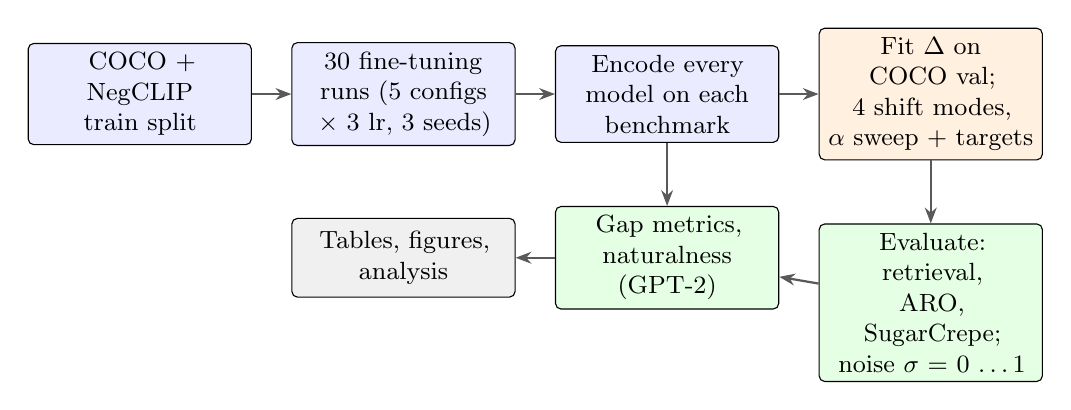
\begin{tikzpicture}[node distance=0.55cm and 0.5cm, every node/.style={font=\small},
  box/.style={draw, rounded corners=2pt, align=center, minimum height=1.0cm, text width=2.6cm, fill=#1},
  box/.default=gray!8, arr/.style={-{Stealth[length=2mm]}, thick, gray!70!black}]
\node[box=blue!8] (data) {COCO + NegCLIP\\train split};
\node[box=blue!8, right=of data] (ft) {30 fine-tuning\\runs (5 configs\\$\times$ 3 lr, 3 seeds)};
\node[box=blue!8, right=of ft] (enc) {Encode every\\model on each\\benchmark};
\node[box=orange!12, right=of enc] (shift) {Fit $\Delta$ on COCO val;\\4 shift modes,\\$\alpha$ sweep + targets};
\node[box=green!10, below=0.8cm of shift] (eval) {Evaluate: retrieval,\\ARO, \mbox{SugarCrepe};\\noise $\sigma$ = 0 \ldots 1};
\node[box=green!10, below=0.8cm of enc] (gap) {Gap metrics,\\naturalness\\(GPT-2)};
\node[box=gray!12, left=of gap] (ana) {Tables, figures,\\analysis};
\draw[arr] (data) -- (ft); \draw[arr] (ft) -- (enc); \draw[arr] (enc) -- (shift);
\draw[arr] (shift) -- (eval); \draw[arr] (enc) -- (gap); \draw[arr] (eval) -- (gap);
\draw[arr] (gap) -- (ana);
\end{tikzpicture}
\caption{Experimental pipeline. Encoding happens once per model and benchmark; every shift, noise level
and metric is computed from the cached embeddings.}
\label{fig:pipeline}
\end{figure}

%=====================================================================
\section{Results}

\subsection{Sanity checks}
Our pipeline reproduces every published number we could check (Table~\ref{tab:sanity}). Our one-file
NegCLIP reproduction at lr $10^{-6}$ matches the released checkpoint on all three ARO tasks to within 0.013.

\begin{table}[H]
\centering\small
\caption{Reproduction of published numbers.}
\label{tab:sanity}
\begin{tabular}{@{}lll@{}}
\toprule
Check & Ours & Published\\
\midrule
CLIP gap $\lVert\gapv\rVert$, COCO & 0.832 & 0.82 \cite{liang}\\
CLIP COCO 5k i2t / t2i R@1 & 0.502 / 0.302 & 0.502 / 0.304 \cite{clip}\\
CLIP VG-Rel / VG-Attr / COCO-Order & 0.638 / 0.632 / 0.472 & 0.59--0.63 / 0.62 / 0.46 \cite{aro}\\
Released NegCLIP VG-Rel / VG-Attr / COCO-Order & 0.838 / 0.721 / 0.825 & 0.81 / 0.71 / 0.86 \cite{aro}\\
FT NegCLIP recipe (lr $10^{-6}$) vs released NegCLIP & 0.840 / 0.725 / 0.838 & 0.838 / 0.721 / 0.825\\
\bottomrule
\end{tabular}
\end{table}

The one mismatch, NegCLIP's COCO-Order (0.825 vs 0.86), is an evaluation detail: NegCLIP was trained
with QuickGELU, but the ARO repository evaluates it with standard GELU. With GELU we obtain 0.868,
matching the paper; that mismatch costs 2--3 points on VG-Relation, VG-Attribution and retrieval. We
report the QuickGELU model throughout and keep the GELU variant as an extra reference.

\subsection{How fine-tuning moves the gap}

\begin{figure}[H]
\centering
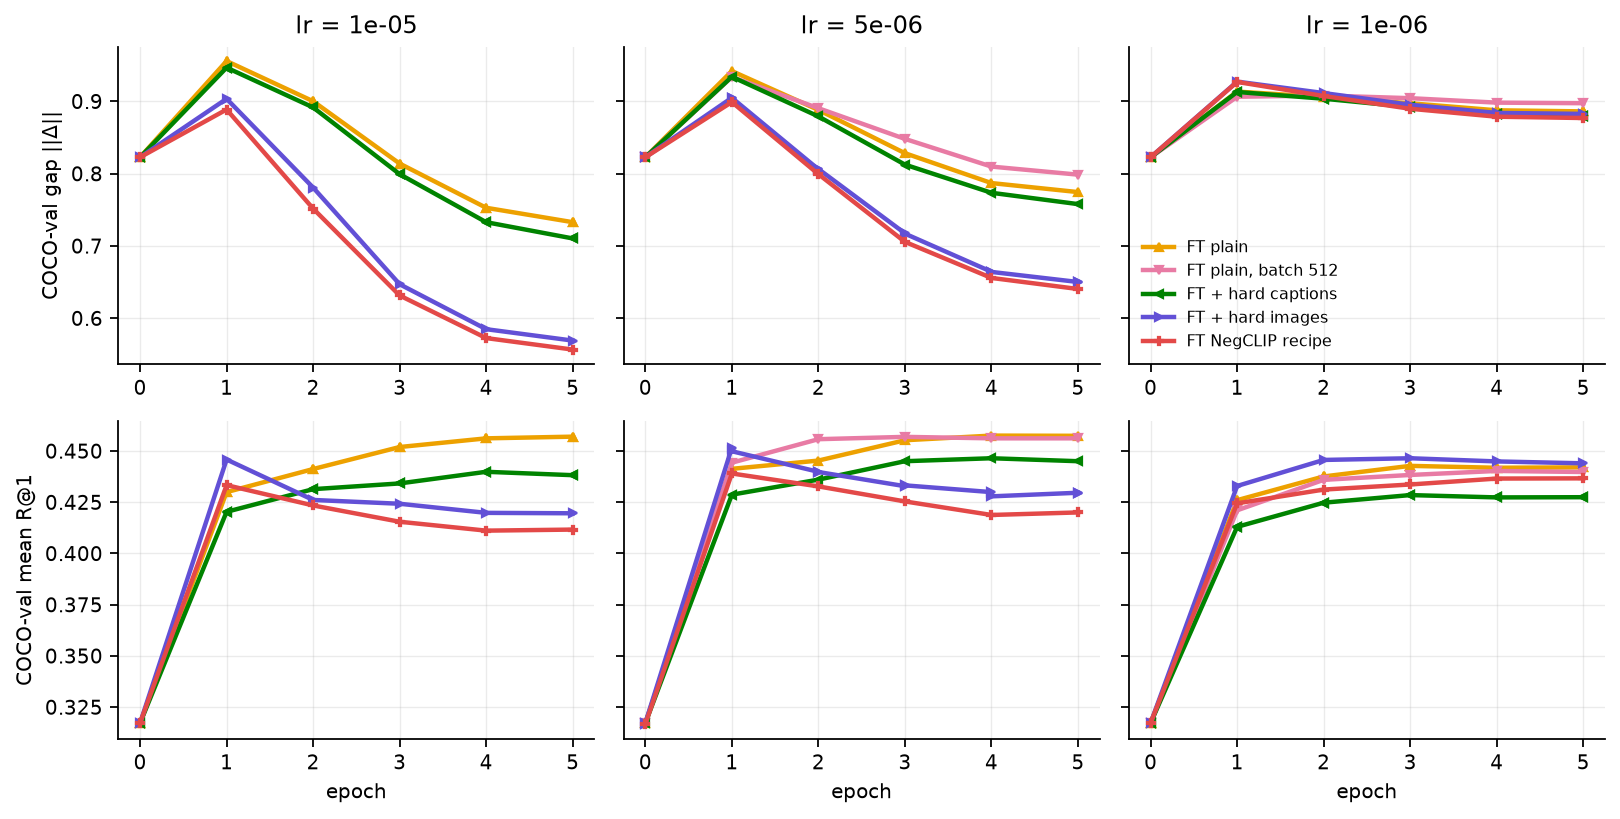
\includegraphics[width=\linewidth]{fig_training_curves.png}
\caption{Validation gap (top) and mean Recall@1 (bottom) over 5 epochs for every configuration and
learning rate (seed 0). Every configuration first widens the gap, then shrinks it; the two
configurations with hard negative images shrink it most.}
\label{fig:training}
\end{figure}

Figure~\ref{fig:training} and Table~\ref{tab:valgap} show three effects:
\begin{enumerate}
\item \textbf{The first epoch always widens the gap} (0.82 $\to$ 0.89--0.96) before it shrinks again.
\item \textbf{Hard negative images shrink the gap.} At lr $5\times10^{-6}$ the final gap is 0.650 with
hard images and 0.640 with the NegCLIP recipe, versus 0.775 for plain fine-tuning and 0.758 with hard
captions. At $10^{-5}$ the ordering is the same (0.569 / 0.557 vs 0.733 / 0.710).
\item \textbf{The learning rate sets how far the gap moves.} At $10^{-6}$ all configurations end at
0.877--0.897, almost where they started.
\end{enumerate}

\begin{table}[H]
\centering\small
\caption{Final-epoch validation gap and mean Recall@1 (seed 0). The batch-512 control was not run at $10^{-5}$.}
\label{tab:valgap}
\begin{tabular}{@{}lcccccc@{}}
\toprule
& \multicolumn{3}{c}{Validation gap $\lVert\gapv\rVert$} & \multicolumn{3}{c}{Validation mean R@1}\\
\cmidrule(lr){2-4}\cmidrule(lr){5-7}
Configuration & $10^{-6}$ & $5\times10^{-6}$ & $10^{-5}$ & $10^{-6}$ & $5\times10^{-6}$ & $10^{-5}$\\
\midrule
FT plain & 0.886 & 0.775 & 0.733 & 0.442 & 0.457 & 0.457\\
FT plain, batch 512 & 0.897 & 0.799 & -- & 0.440 & 0.456 & --\\
FT + hard captions & 0.880 & 0.758 & 0.710 & 0.427 & 0.445 & 0.438\\
FT + hard images & 0.883 & \textbf{0.650} & \textbf{0.569} & 0.444 & 0.430 & 0.420\\
FT NegCLIP recipe & 0.877 & \textbf{0.640} & \textbf{0.557} & 0.437 & 0.420 & 0.412\\
\bottomrule
\end{tabular}
\end{table}

\paragraph{Batch-size control.}
Hard negative images double the batch, so the gap reduction could come from the larger batch rather
than from harder negatives. The batch-512 control rules this out (Table~\ref{tab:batch}): with 512
random pairs the gap ends at 0.799, \emph{larger} than plain fine-tuning (0.775) and far from the hard-image
models (0.650). On every benchmark the control stays within 0.015 of plain fine-tuning.

\begin{table}[H]
\centering\small
\caption{Batch-size control (seed 0). Only the hard negative images, not the batch size, shrink the gap.}
\label{tab:batch}
\begin{tabular}{@{}llcccccc@{}}
\toprule
Configuration & lr & Val gap & i2t R@1 & t2i R@1 & COCO-Order & VG-Rel & VG-Attr\\
\midrule
FT plain & $5\times10^{-6}$ & 0.775 & 0.618 & 0.454 & 0.291 & 0.542 & 0.647\\
FT plain, batch 512 & $5\times10^{-6}$ & 0.799 & 0.623 & 0.460 & 0.292 & 0.556 & 0.643\\
FT + hard images & $5\times10^{-6}$ & \textbf{0.650} & 0.586 & 0.437 & 0.266 & 0.543 & 0.633\\
\midrule
FT plain & $10^{-6}$ & 0.886 & 0.615 & 0.446 & 0.336 & 0.592 & 0.652\\
FT plain, batch 512 & $10^{-6}$ & 0.897 & 0.615 & 0.444 & 0.347 & 0.602 & 0.653\\
FT + hard images & $10^{-6}$ & 0.883 & 0.607 & 0.451 & 0.303 & 0.554 & 0.650\\
\bottomrule
\end{tabular}
\end{table}

\subsection{Compositional accuracy at matched learning rates}

\begin{figure}[H]
\centering
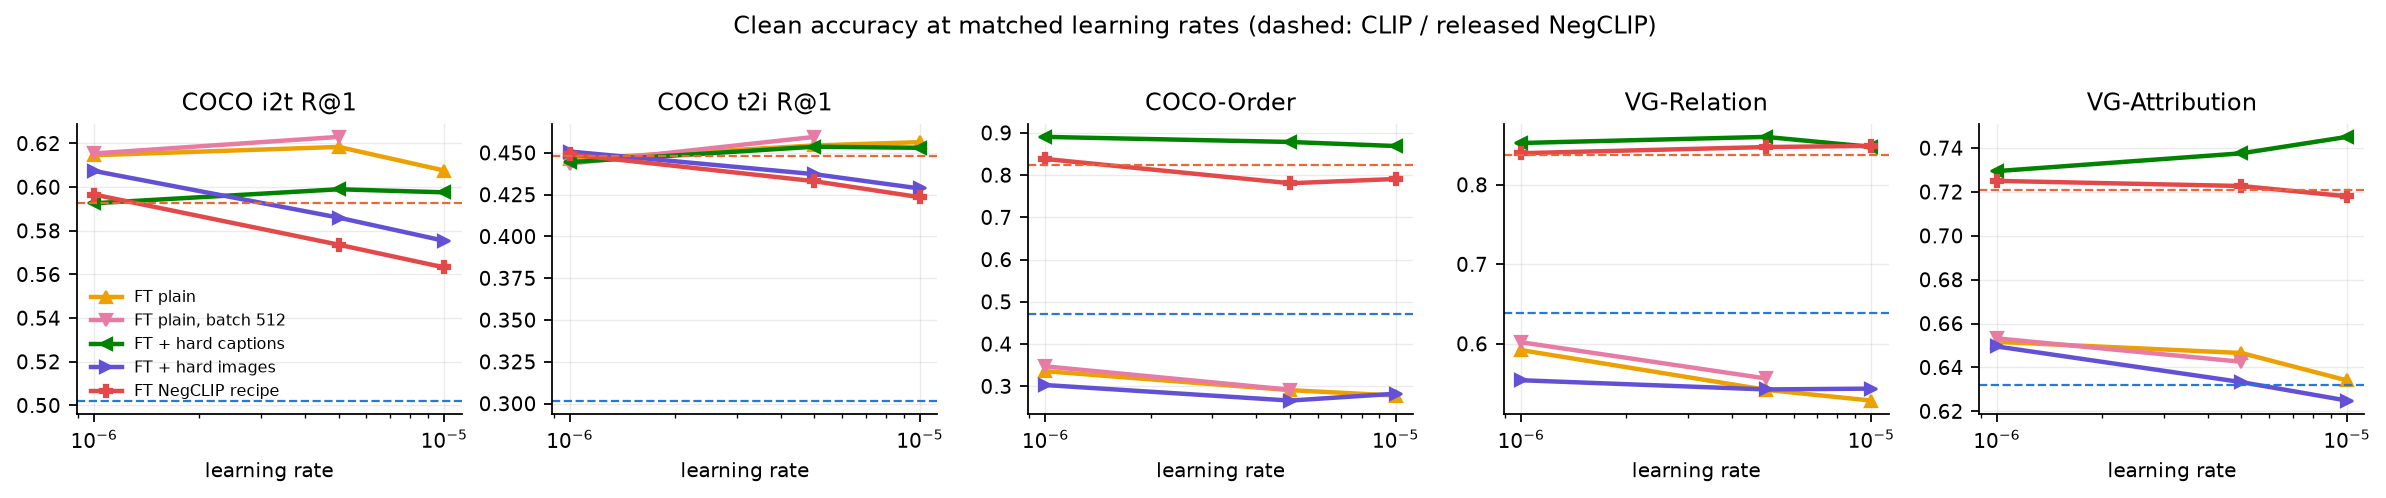
\includegraphics[width=\linewidth]{fig_matched_lr.png}
\caption{Clean accuracy of every configuration at every learning rate (seed 0). Dashed lines: CLIP
and released NegCLIP. The ranking of configurations is the same at every learning rate.}
\label{fig:matchedlr}
\end{figure}

\begin{table}[H]
\centering\small
\caption{Clean accuracy at matched learning rates (seed 0). Best compositional score per learning rate in bold.}
\label{tab:matched}
\begin{tabular}{@{}llccccc@{}}
\toprule
Configuration & lr & i2t R@1 & t2i R@1 & COCO-Order & VG-Relation & VG-Attribution\\
\midrule
CLIP & -- & 0.502 & 0.302 & 0.472 & 0.638 & 0.632\\
NegCLIP (released) & -- & 0.593 & 0.448 & 0.825 & 0.838 & 0.721\\
\midrule
FT plain & $10^{-6}$ & 0.615 & 0.446 & 0.336 & 0.592 & 0.652\\
FT plain, batch 512 & $10^{-6}$ & 0.615 & 0.444 & 0.347 & 0.602 & 0.653\\
FT + hard captions & $10^{-6}$ & 0.593 & 0.444 & \textbf{0.890} & \textbf{0.852} & \textbf{0.729}\\
FT + hard images & $10^{-6}$ & 0.607 & 0.451 & 0.303 & 0.554 & 0.650\\
FT NegCLIP recipe & $10^{-6}$ & 0.597 & 0.449 & 0.838 & 0.840 & 0.725\\
\midrule
FT plain & $5\times10^{-6}$ & 0.618 & 0.454 & 0.291 & 0.542 & 0.647\\
FT plain, batch 512 & $5\times10^{-6}$ & 0.623 & 0.460 & 0.292 & 0.556 & 0.643\\
FT + hard captions & $5\times10^{-6}$ & 0.599 & 0.454 & \textbf{0.878} & \textbf{0.860} & \textbf{0.738}\\
FT + hard images & $5\times10^{-6}$ & 0.586 & 0.437 & 0.266 & 0.543 & 0.633\\
FT NegCLIP recipe & $5\times10^{-6}$ & 0.574 & 0.433 & 0.781 & 0.847 & 0.723\\
\midrule
FT plain & $10^{-5}$ & 0.608 & 0.456 & 0.278 & 0.529 & 0.634\\
FT + hard captions & $10^{-5}$ & 0.598 & 0.453 & \textbf{0.869} & 0.848 & \textbf{0.745}\\
FT + hard images & $10^{-5}$ & 0.575 & 0.429 & 0.282 & 0.544 & 0.625\\
FT NegCLIP recipe & $10^{-5}$ & 0.563 & 0.423 & 0.791 & \textbf{0.849} & 0.718\\
\bottomrule
\end{tabular}
\end{table}

Table~\ref{tab:matched} and Figure~\ref{fig:matchedlr} give four results:
\begin{itemize}
\item \textbf{Compositionality comes from hard negative captions.} Only the two configurations with hard
captions become compositional; hard images alone add nothing over plain fine-tuning.
\item \textbf{Hard captions alone are best at every learning rate}, ahead of the released NegCLIP:
COCO-Order 0.87--0.89 (vs 0.825), VG-Relation 0.85--0.86 (vs 0.838), VG-Attribution 0.73--0.745 (vs 0.721).
\item \textbf{Adding hard images to hard captions costs accuracy:} COCO-Order falls from 0.890 to 0.838 at
$10^{-6}$ and from 0.878 to 0.781 at $5\times10^{-6}$, and retrieval drops at the higher learning rates.
\item \textbf{Plain COCO fine-tuning makes the model less order-sensitive than CLIP} (COCO-Order
0.47 $\to$ 0.28--0.35) while improving retrieval by 0.11--0.15 Recall@1.
\end{itemize}
Because the ranking is identical at all three learning rates, the learning-rate confound of the
mid-project report (configurations selected at different learning rates) does not change any conclusion.

\paragraph{Seed variance.}
Across three seeds the standard deviation is at most 0.007 on every metric (Table~\ref{tab:seeds},
Figure~\ref{fig:seeds}); the differences between configurations are 10--60 times larger.

\begin{figure}[H]
\centering
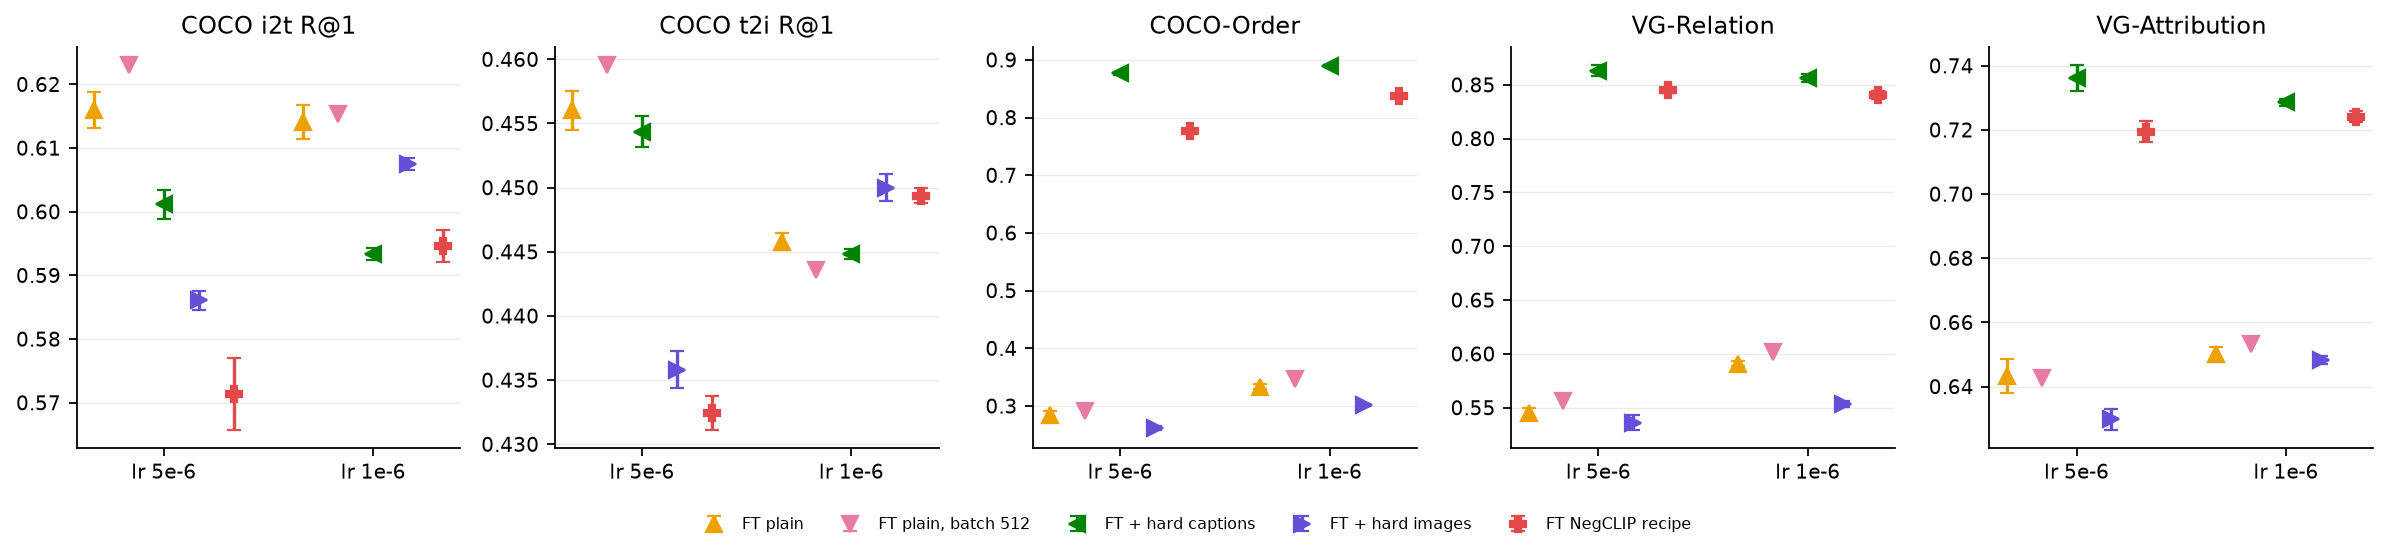
\includegraphics[width=\linewidth]{fig_seed_variance.png}
\caption{Mean and standard deviation over seeds 0, 1, 2 at learning rates $10^{-6}$ and $5\times10^{-6}$.
Error bars are barely visible because seed noise is below 0.007.}
\label{fig:seeds}
\end{figure}

\begin{table}[H]
\centering\small
\caption{Mean $\pm$ standard deviation over three seeds.}
\label{tab:seeds}
\begin{tabular}{@{}llccccc@{}}
\toprule
Configuration & lr & i2t R@1 & t2i R@1 & COCO-Order & VG-Relation & VG-Attribution\\
\midrule
FT plain & $10^{-6}$ & .614$\pm$.003 & .446$\pm$.001 & .333$\pm$.005 & .591$\pm$.002 & .650$\pm$.002\\
FT + hard captions & $10^{-6}$ & .593$\pm$.001 & .445$\pm$.000 & .890$\pm$.001 & .856$\pm$.004 & .729$\pm$.001\\
FT + hard images & $10^{-6}$ & .607$\pm$.001 & .450$\pm$.001 & .301$\pm$.001 & .553$\pm$.003 & .648$\pm$.001\\
FT NegCLIP recipe & $10^{-6}$ & .595$\pm$.003 & .449$\pm$.001 & .838$\pm$.001 & .841$\pm$.004 & .724$\pm$.002\\
\midrule
FT plain & $5\times10^{-6}$ & .616$\pm$.003 & .456$\pm$.002 & .284$\pm$.007 & .545$\pm$.005 & .643$\pm$.005\\
FT + hard captions & $5\times10^{-6}$ & .601$\pm$.002 & .454$\pm$.001 & .877$\pm$.002 & .863$\pm$.005 & .736$\pm$.004\\
FT + hard images & $5\times10^{-6}$ & .586$\pm$.002 & .436$\pm$.001 & .262$\pm$.003 & .536$\pm$.007 & .630$\pm$.003\\
FT NegCLIP recipe & $5\times10^{-6}$ & .571$\pm$.006 & .432$\pm$.001 & .777$\pm$.003 & .845$\pm$.002 & .719$\pm$.003\\
\bottomrule
\end{tabular}
\end{table}

\subsection{Gap geometry}

\begin{figure}[H]
\centering
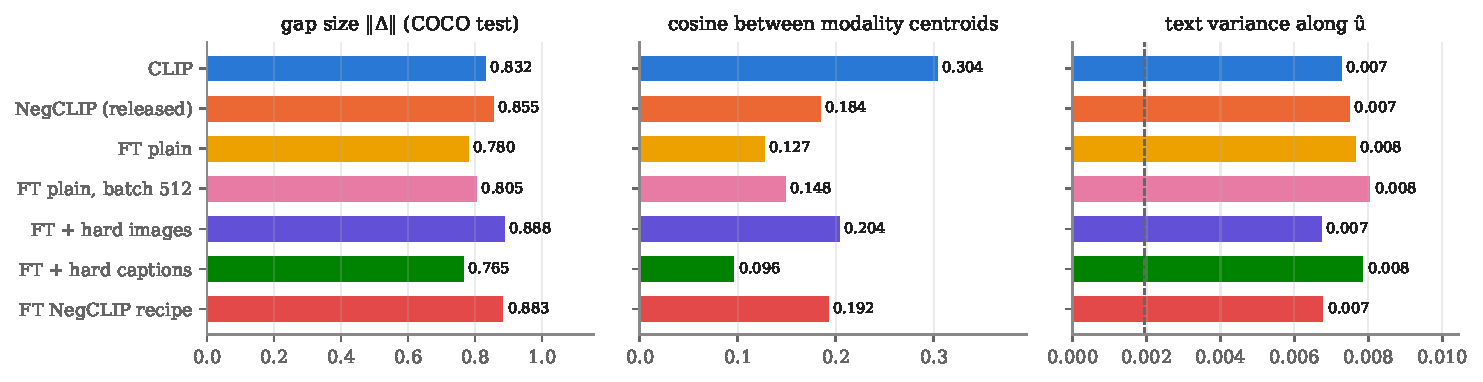
\includegraphics[width=\linewidth]{gap_geometry.pdf}
\caption{Gap geometry on COCO test for the selected checkpoint of each configuration. Right: the
fraction of text variance along $\uhat$; the dashed line marks a random direction ($1/512$).}
\label{fig:geometry}
\end{figure}

Figure~\ref{fig:geometry} and Table~\ref{tab:geometry} summarise the geometry. In every model image and
text embeddings remain perfectly linearly separable, and the gap direction carries only 0.2--0.4\% of
image variance and 0.7--0.8\% of text variance (for text, 3.5--4 times a random direction), so the gap is
\emph{nearly}, but not exactly, orthogonal to how embeddings vary. Fine-tuning spreads the two cones apart in angle (centroid cosine 0.10--0.20 vs 0.30 for CLIP), and
FT + hard captions has the smallest gap of all selected checkpoints (0.765), yet hard captions barely move the gap at matched learning rate. Note that the
selected checkpoints of the hard-image configurations were trained at $10^{-6}$, where the gap barely
moves; the matched-learning-rate effect is in Table~\ref{tab:valgap}.

\begin{table}[H]
\centering\small
\caption{Gap metrics on COCO test (selected checkpoints).}
\label{tab:geometry}
\resizebox{\linewidth}{!}{\begin{tabular}{@{}lcccccc@{}}
\toprule
Model & $\lVert\gapv\rVert$ & Centroid cos & Matched cos & Var.\ along $\uhat$ (img) & Var.\ along $\uhat$ (txt) & Lin.\ sep.\\
\midrule
CLIP & 0.832 & 0.304 & 0.303 & 0.004 & 0.007 & 1.000\\
NegCLIP (released) & 0.855 & 0.184 & 0.292 & 0.003 & 0.007 & 1.000\\
NegCLIP (GELU) & 0.903 & 0.208 & 0.286 & 0.002 & 0.006 & 1.000\\
FT plain & 0.780 & 0.127 & 0.297 & 0.003 & 0.008 & 1.000\\
FT plain, batch 512 & 0.805 & 0.148 & 0.297 & 0.003 & 0.008 & 1.000\\
FT + hard captions & 0.765 & 0.096 & 0.292 & 0.003 & 0.008 & 1.000\\
FT + hard images & 0.888 & 0.204 & 0.297 & 0.002 & 0.007 & 1.000\\
FT NegCLIP recipe & 0.883 & 0.192 & 0.293 & 0.002 & 0.007 & 1.000\\
\bottomrule
\end{tabular}}
\end{table}

\paragraph{Gap size does not predict compositional skill.}
Plotting every seed-0 run's compositional accuracy against its final gap (Figure~\ref{fig:gapskill})
shows two horizontal bands: runs with hard captions score 0.78--0.89 on COCO-Order at every gap from
0.56 to 0.88, and runs without them score 0.27--0.35 over the same range. The gap is set by hard images
and the learning rate; compositional skill is set by hard captions.

\begin{figure}[H]
\centering
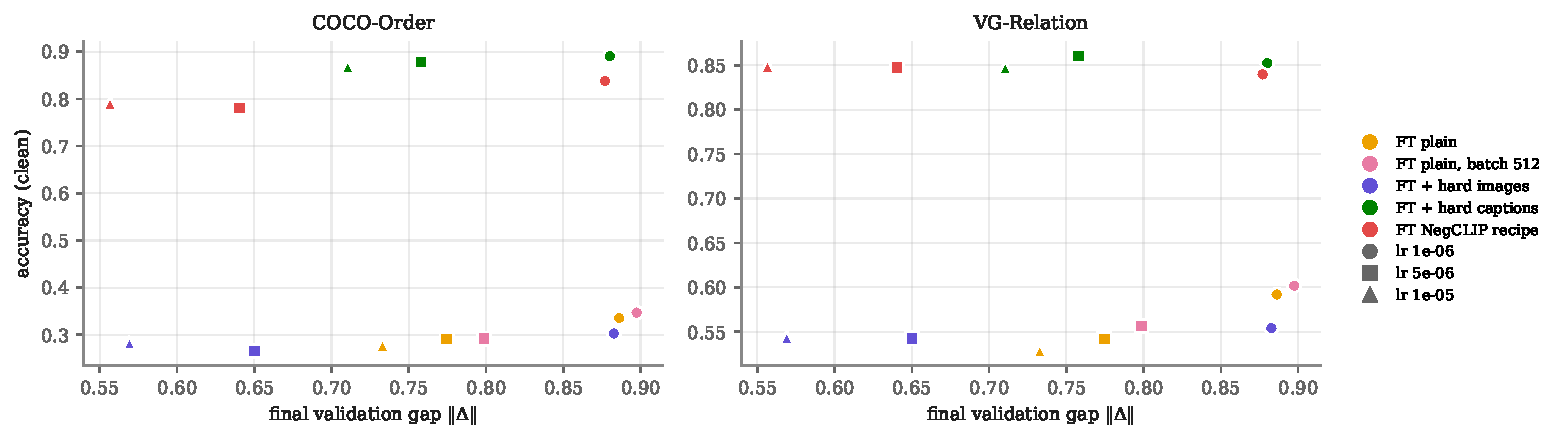
\includegraphics[width=0.95\linewidth]{gap_vs_skill.pdf}
\caption{Clean compositional accuracy vs final validation gap for every seed-0 run. Colour: configuration;
marker: learning rate.}
\label{fig:gapskill}
\end{figure}

\subsection{Closing the gap post hoc}

\begin{figure}[H]
\centering
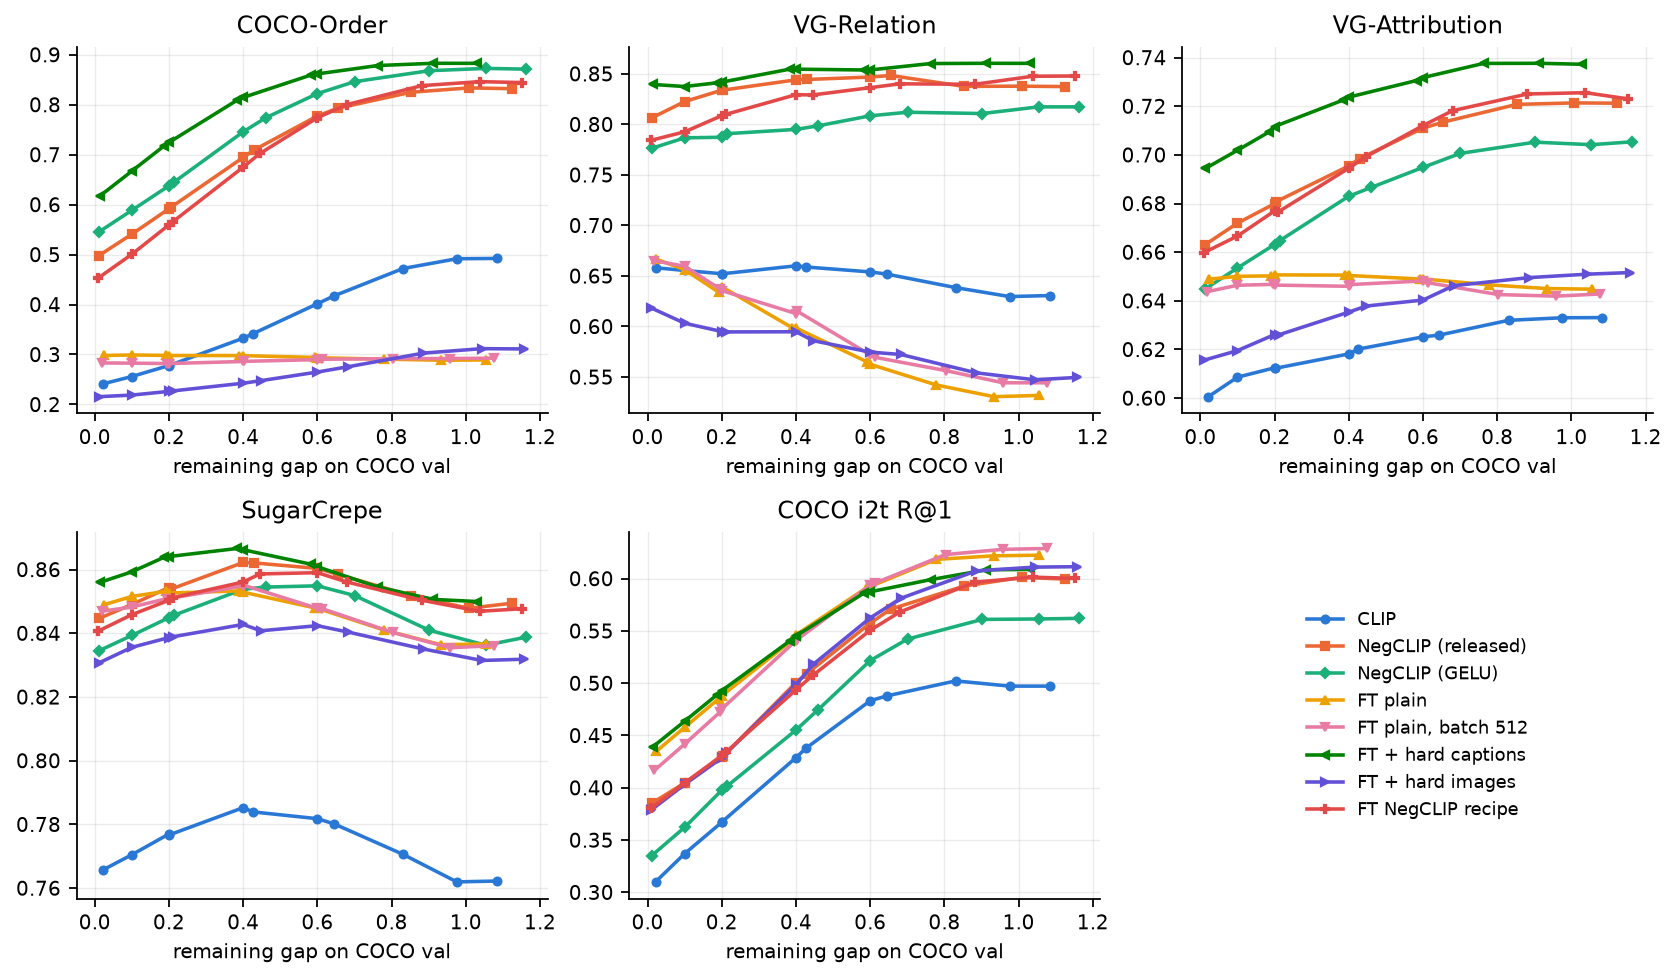
\includegraphics[width=\linewidth]{fig_shift_text_mean.png}
\caption{Accuracy as a function of the remaining gap on COCO val (text shift, mean $\gapv$, no noise).
Points to the right of each model's original gap (0.76--0.90) widen the gap ($\alpha<0$); moving left closes it.}
\label{fig:shift}
\end{figure}

Figure~\ref{fig:shift} traces accuracy as the gap is closed, and Figure~\ref{fig:closingbars} shows the
change when the remaining gap is shrunk from about 0.85 to 0.10.

\begin{figure}[H]
\centering
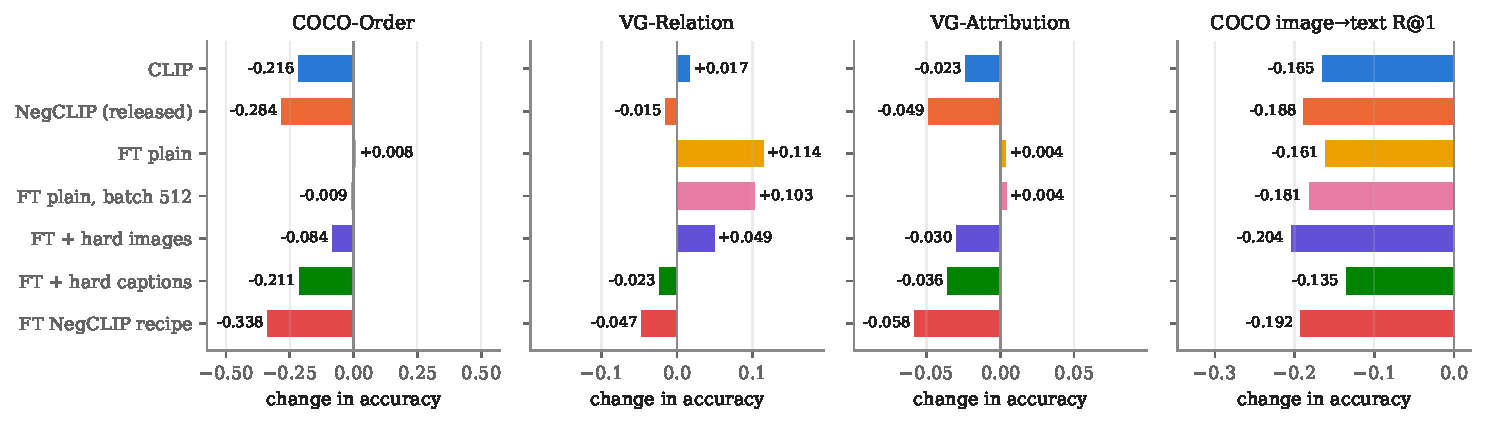
\includegraphics[width=\linewidth]{gap_closing_bars.pdf}
\caption{Change in clean accuracy from closing the gap to 0.10 (text shift, mean $\gapv$).}
\label{fig:closingbars}
\end{figure}

\begin{table}[H]
\centering\small
\caption{Change in clean accuracy when the remaining gap on COCO val is shrunk to 0.10 (text shift, mean $\gapv$).}
\label{tab:closing}
\resizebox{\linewidth}{!}{\begin{tabular}{@{}lcccccc@{}}
\toprule
Model & Gap before & COCO-Order & VG-Relation & VG-Attribution & SugarCrepe & i2t R@1\\
\midrule
CLIP & 0.831 & \negc{$-$0.216} & $+$0.017 & \negc{$-$0.023} & $-$0.000 & \negc{$-$0.165}\\
NegCLIP (released) & 0.853 & \negc{$-$0.284} & $-$0.015 & \negc{$-$0.049} & $-$0.003 & \negc{$-$0.188}\\
NegCLIP (GELU) & 0.902 & \negc{$-$0.279} & $-$0.024 & \negc{$-$0.052} & $-$0.002 & \negc{$-$0.199}\\
FT plain & 0.779 & $+$0.008 & \pos{$+$0.114} & $+$0.004 & $+$0.011 & \negc{$-$0.161}\\
FT plain, batch 512 & 0.803 & $-$0.009 & \pos{$+$0.103} & $+$0.004 & $+$0.008 & \negc{$-$0.181}\\
FT + hard captions & 0.763 & \negc{$-$0.211} & $-$0.023 & \negc{$-$0.036} & $+$0.005 & \negc{$-$0.135}\\
FT + hard images & 0.886 & \negc{$-$0.084} & \pos{$+$0.049} & \negc{$-$0.030} & $+$0.001 & \negc{$-$0.204}\\
FT NegCLIP recipe & 0.881 & \negc{$-$0.338} & \negc{$-$0.047} & \negc{$-$0.058} & $-$0.005 & \negc{$-$0.192}\\
\bottomrule
\end{tabular}}
\end{table}

\begin{itemize}
\item \textbf{Every model with hard captions loses} 0.21--0.34 on COCO-Order and 0.04--0.06 on
VG-Attribution. Our NegCLIP recipe loses most ($-0.338$), dropping from 0.838 to 0.50.
\item \textbf{Retrieval drops for every model} by 0.13--0.20 Recall@1: the original gap is close to
optimal for retrieval.
\item \textbf{The only gains are on VG-Relation, and only without hard captions} (FT plain $+0.114$,
batch 512 $+0.103$, hard images $+0.049$). These models start near or below CLIP on that benchmark.
\item \textbf{The symmetric ``both'' shift hurts more} than the text shift
(released NegCLIP COCO-Order $-0.387$ vs $-0.327$ at $\alpha=1$), and mean and median $\gapv$ differ by at most 0.01.
\item \textbf{Widening the gap} ($\alpha<0$) changes accuracy by at most 0.08 in either direction and never turns a loss into a clear gain.
\item \textbf{Pooled SugarCrepe} peaks slightly (about $+0.01$ to $+0.02$) at a remaining gap near 0.4 and returns to the starting level at 0.1; Section~\ref{sec:sc} shows this hides large opposite changes between subsets.
\end{itemize}

\subsection{Why closing the gap hurts: the mechanism}

\paragraph{Without re-normalisation the shift does nothing.}
For a fixed image $x$, the text shift without re-normalisation changes each caption's score from
$x^\top y$ to $x^\top y+\alpha\,x^\top\gapv$. The added term is the same for every candidate caption, so
rankings cannot change. Empirically, the \textbf{text\_norenorm} shift leaves every accuracy unchanged to
four decimals for all 8 models on all 4 case benchmarks (grey bars in Figure~\ref{fig:mechanism}, green
lines in Figure~\ref{fig:h3}). Any effect of the shift therefore comes from re-normalisation.

\paragraph{Re-normalisation acts on one coordinate.}
Decompose each caption as $y=y_\perp+(m+d)\,\uhat$, where $m$ is the mean projection of all captions on
$\uhat$ and $d$ is the caption's own deviation. With re-normalisation the shifted score is
\begin{equation}
s'(x,y)=\frac{x^\top y+\alpha\,x^\top\gapv}{\lVert y+\alpha\gapv\rVert},\qquad
\lVert y+\alpha\gapv\rVert^2=1+2\alpha\lVert\gapv\rVert(m+d)+\alpha^2\lVert\gapv\rVert^2 .
\end{equation}
The numerator gains a large shared constant, and the denominator differs between captions only through
$d$. Closing the gap therefore re-weights captions by their position along $\uhat$, and the
re-weighting largely cancels the contribution of $d$ to the score. The \textbf{orth} control tests this
directly: at $\alpha=0$ it applies \emph{no shift at all} and only removes $d$.

\begin{figure}[H]
\centering
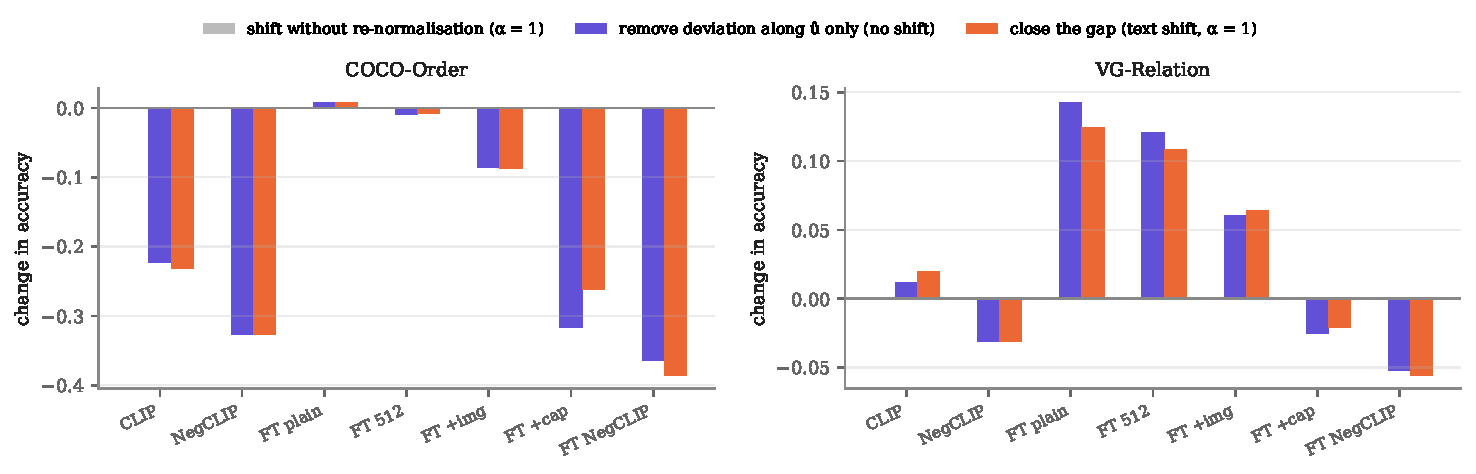
\includegraphics[width=\linewidth]{mechanism_bars.pdf}
\caption{Change in accuracy from three interventions. Grey (shift without re-normalisation) is exactly
zero for every model. Removing only each caption's deviation along $\uhat$ (purple) reproduces the effect
of closing the gap (orange).}
\label{fig:mechanism}
\end{figure}

\begin{table}[H]
\centering\small
\caption{Removing the deviation along $\uhat$ alone (orth, $\alpha=0$) vs closing the gap (text, $\alpha=1$).}
\label{tab:mechanism}
\begin{tabular}{@{}lcccc@{}}
\toprule
& \multicolumn{2}{c}{COCO-Order} & \multicolumn{2}{c}{VG-Relation}\\
\cmidrule(lr){2-3}\cmidrule(lr){4-5}
Model & remove $d$ only & close gap & remove $d$ only & close gap\\
\midrule
CLIP & $-$0.223 & $-$0.231 & $+$0.012 & $+$0.020\\
NegCLIP (released) & $-$0.327 & $-$0.327 & $-$0.031 & $-$0.031\\
NegCLIP (GELU) & $-$0.281 & $-$0.323 & $-$0.032 & $-$0.034\\
FT plain & $+$0.008 & $+$0.007 & $+$0.143 & $+$0.125\\
FT plain, batch 512 & $-$0.010 & $-$0.009 & $+$0.121 & $+$0.109\\
FT + hard captions & $-$0.316 & $-$0.261 & $-$0.025 & $-$0.021\\
FT + hard images & $-$0.086 & $-$0.087 & $+$0.061 & $+$0.064\\
FT NegCLIP recipe & $-$0.364 & $-$0.385 & $-$0.052 & $-$0.056\\
\bottomrule
\end{tabular}
\end{table}

Table~\ref{tab:mechanism} shows that removing $d$ alone matches the full gap-closing change almost
exactly: $-0.327$ vs $-0.327$ for released NegCLIP on COCO-Order, $-0.364$ vs $-0.385$ for our NegCLIP
recipe, and $+0.143$ vs $+0.125$ for FT plain on VG-Relation. Once $d$ has been removed, shifting further
changes far less than the original shift did (compare the slopes of the orth and text curves in Figure~\ref{fig:h3}).
\textbf{Closing the gap is, in effect, deleting one direction from the text embeddings.}

\begin{figure}[H]
\centering
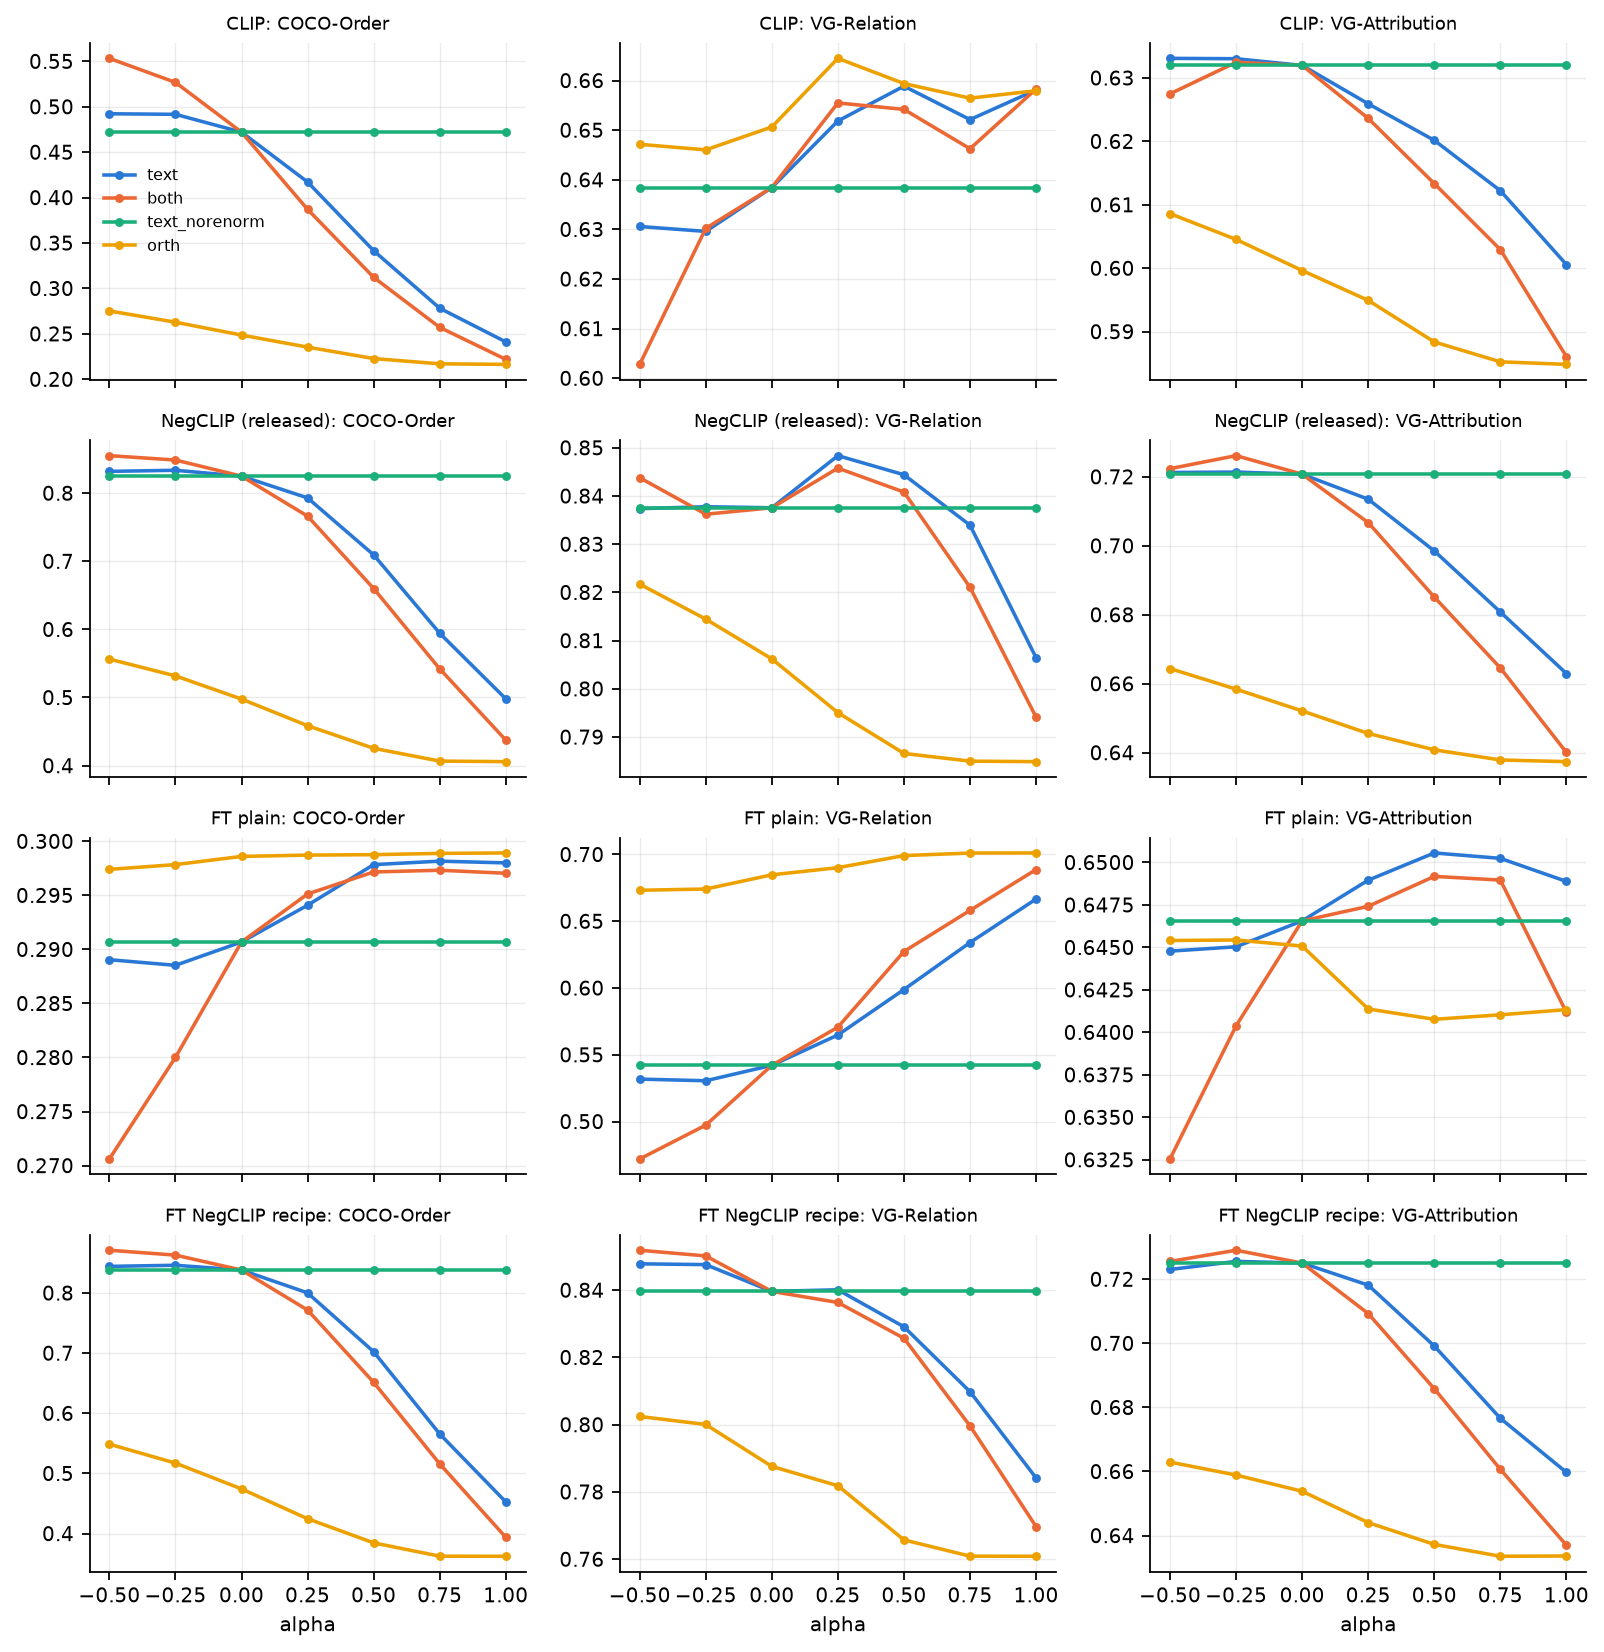
\includegraphics[width=0.92\linewidth]{fig_h3_controls.png}
\caption{Accuracy vs $\alpha$ for the four shift modes on four representative models. text\_norenorm
(green) is flat by construction. orth (yellow) starts lower at $\alpha=0$ because it already removes the
deviation along $\uhat$, and then changes little.}
\label{fig:h3}
\end{figure}

\paragraph{That direction carries compositional information.}
The deviation along $\uhat$ holds only about 0.7\% of the text variance (Table~\ref{tab:geometry}), yet
removing it costs hard-caption models 0.28--0.36 on COCO-Order and 0.06--0.07 on VG-Attribution. In
models trained with hard captions, the coordinate along the gap direction helps tell the true caption
from its word-shuffled or attribute-swapped versions. In models without hard captions the same
coordinate works \emph{against} VG-Relation, which is why only they gain there. This refutes H3 for
order and attribute tasks: a uniform text shift is harmless only without re-normalisation.

\subsection{SugarCrepe}\label{sec:sc}

\begin{figure}[H]
\centering
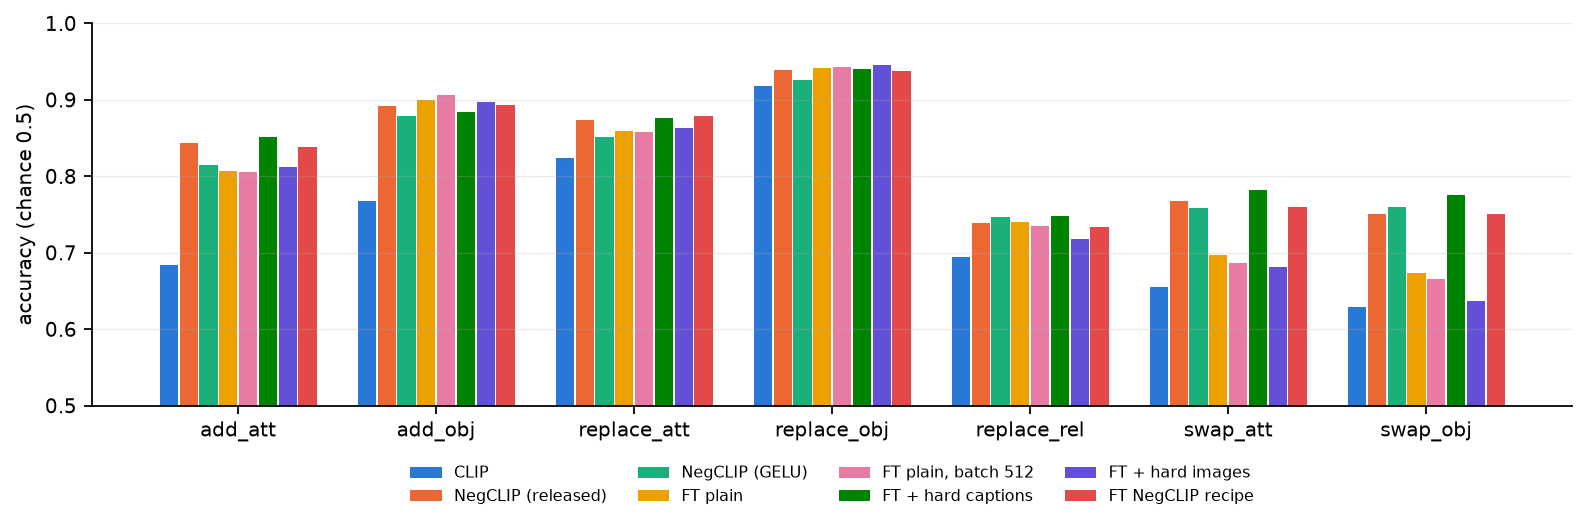
\includegraphics[width=\linewidth]{fig_sugarcrepe.png}
\caption{Clean SugarCrepe accuracy per subset.}
\label{fig:sc}
\end{figure}

\begin{table}[H]
\centering\small
\caption{Clean SugarCrepe accuracy per subset and mean over subsets.}
\label{tab:scclean}
\resizebox{\linewidth}{!}{\begin{tabular}{@{}lcccccccc@{}}
\toprule
Model & add\_att & add\_obj & repl\_att & repl\_obj & repl\_rel & swap\_att & swap\_obj & mean\\
\midrule
CLIP & 0.684 & 0.767 & 0.824 & 0.918 & 0.695 & 0.655 & 0.629 & 0.739\\
NegCLIP (released) & 0.844 & 0.892 & 0.873 & 0.939 & 0.739 & 0.767 & 0.751 & 0.829\\
FT plain & 0.806 & 0.900 & 0.859 & 0.942 & 0.740 & 0.697 & 0.673 & 0.803\\
FT plain, batch 512 & 0.805 & 0.906 & 0.858 & 0.942 & 0.735 & 0.686 & 0.665 & 0.800\\
FT + hard captions & \textbf{0.851} & 0.884 & 0.876 & 0.941 & \textbf{0.748} & \textbf{0.782} & \textbf{0.776} & \textbf{0.837}\\
FT + hard images & 0.812 & 0.897 & 0.863 & \textbf{0.946} & 0.718 & 0.682 & 0.637 & 0.793\\
FT NegCLIP recipe & 0.838 & 0.894 & \textbf{0.879} & 0.938 & 0.733 & 0.760 & 0.751 & 0.828\\
\bottomrule
\end{tabular}}
\end{table}

\textbf{Clean} (Table~\ref{tab:scclean}, Figure~\ref{fig:sc}): plain COCO fine-tuning already lifts the
\emph{add} and \emph{replace} subsets; hard captions are what lift the \emph{swap} subsets
(swap\_att 0.70 $\to$ 0.78, swap\_obj 0.67 $\to$ 0.78), and hard images add nothing there. The ranking
by mean accuracy is FT + hard captions (0.837) $>$ released NegCLIP (0.829) $\approx$ FT NegCLIP recipe
(0.828) $>$ FT plain (0.803) $>$ CLIP (0.739), matching ARO.

\begin{figure}[H]
\centering
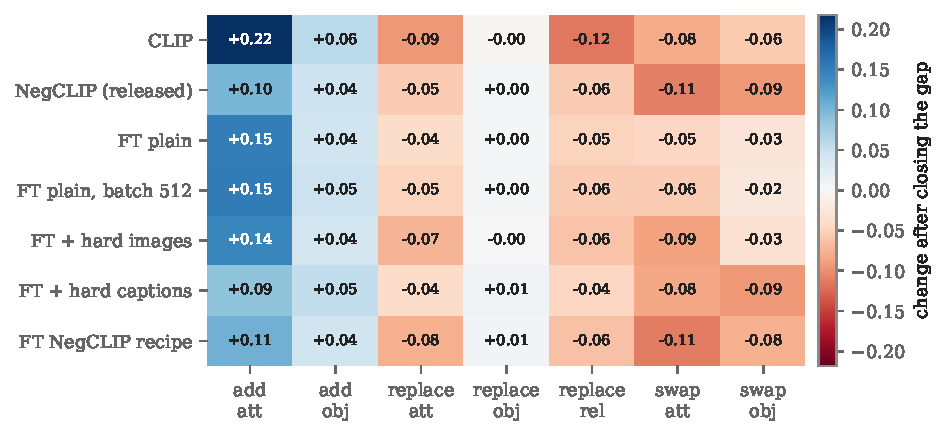
\includegraphics[width=0.78\linewidth]{sugarcrepe_heatmap.pdf}
\caption{Change in SugarCrepe accuracy per subset after closing the gap ($\alpha=1$, text shift). Blue:
gain; red: loss.}
\label{fig:scheat}
\end{figure}

\textbf{After closing the gap} (Figure~\ref{fig:scheat}): accuracy rises on \texttt{add\_att}
($+0.09$ to $+0.22$) and \texttt{add\_obj} ($+0.04$ to $+0.06$) for every model, and falls on
\texttt{replace\_att}, \texttt{replace\_rel} and both \texttt{swap} subsets ($-0.03$ to $-0.11$).
\texttt{replace\_obj} does not move. The gains and losses cancel to about zero in the pooled score
(Table~\ref{tab:closing}). The \emph{add} negatives are longer than their positives, so one plausible reading
is that the coordinate along $\uhat$ correlates with caption length, and removing it removes a length
bias that the add negatives exploit.

\subsection{Robustness to embedding noise}

\begin{figure}[H]
\centering
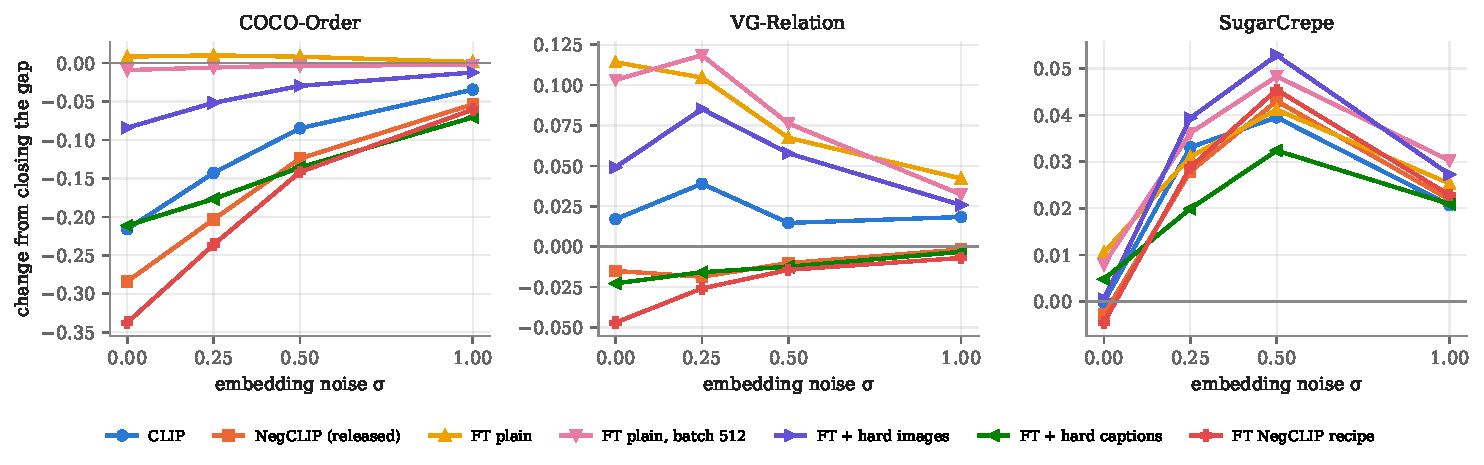
\includegraphics[width=\linewidth]{noise_lines.pdf}
\caption{Change in accuracy from closing the gap (to 0.10) at each noise level $\sigma$. The damage on
COCO-Order shrinks as noise grows; on SugarCrepe, closing the gap helps every model under noise.}
\label{fig:noise}
\end{figure}

\begin{table}[H]
\centering\small
\caption{Change from closing the gap at each noise level $\sigma$ (mean of 3 noise seeds).}
\label{tab:noise}
\begin{tabular}{@{}lcccccccc@{}}
\toprule
& \multicolumn{4}{c}{COCO-Order} & \multicolumn{4}{c}{SugarCrepe}\\
\cmidrule(lr){2-5}\cmidrule(lr){6-9}
Model & $\sigma$=0 & 0.25 & 0.5 & 1.0 & 0 & 0.25 & 0.5 & 1.0\\
\midrule
CLIP & $-$.216 & $-$.143 & $-$.085 & $-$.034 & .000 & $+$.033 & $+$.040 & $+$.021\\
NegCLIP (released) & $-$.284 & $-$.203 & $-$.124 & $-$.054 & $-$.003 & $+$.028 & $+$.043 & $+$.022\\
FT plain & $+$.008 & $+$.010 & $+$.008 & $+$.002 & $+$.011 & $+$.031 & $+$.041 & $+$.025\\
FT plain, batch 512 & $-$.009 & $-$.006 & $-$.003 & $-$.003 & $+$.008 & $+$.036 & $+$.048 & $+$.030\\
FT + hard captions & $-$.211 & $-$.177 & $-$.136 & $-$.071 & $+$.005 & $+$.020 & $+$.032 & $+$.021\\
FT + hard images & $-$.084 & $-$.052 & $-$.030 & $-$.012 & $+$.001 & $+$.039 & $+$.053 & $+$.027\\
FT NegCLIP recipe & $-$.338 & $-$.236 & $-$.142 & $-$.060 & $-$.005 & $+$.029 & $+$.045 & $+$.023\\
\bottomrule
\end{tabular}
\end{table}

The harm from closing the gap shrinks steadily as noise grows: for the NegCLIP recipe on COCO-Order it
goes from $-0.338$ without noise to $-0.060$ at $\sigma=1$ (Table~\ref{tab:noise},
Figure~\ref{fig:noise}). On SugarCrepe closing the gap gives a small gain for every model once noise is
present, peaking at $+0.03$ to $+0.05$ at $\sigma=0.5$. The robustness benefit predicted by H2 therefore
appears, but only in the noisy regime, it is no larger for hard-negative models than for the others,
and on clean data it is outweighed by the loss on order and attribute tasks.

\subsection{Is the gap direction a ``naturalness'' direction?}

In the mid-project report we observed that word-shuffled COCO-Order captions tend to lie further along
the text side of $\uhat$ than true captions, and hypothesised that $\uhat$ encodes how natural a caption
reads. We tested this directly with GPT-2 perplexity on all 119,724 COCO-Order captions
(Table~\ref{tab:nat}, Figure~\ref{fig:nat}).

\begin{figure}[H]
\centering
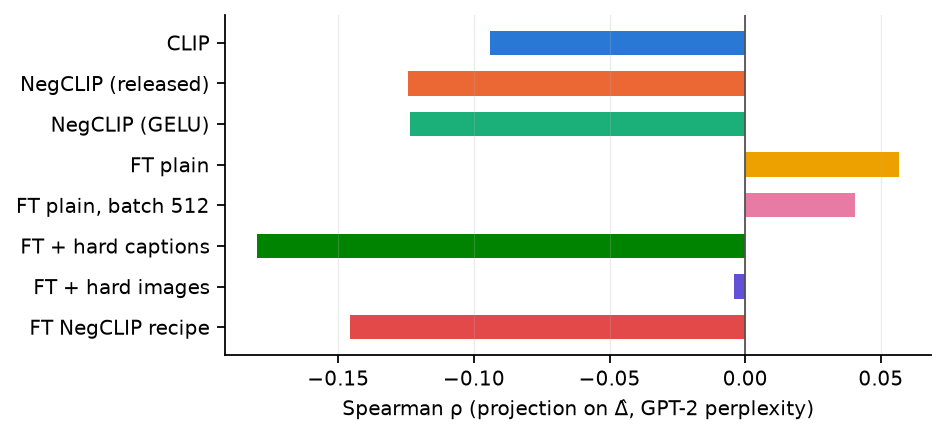
\includegraphics[width=0.6\linewidth]{fig_naturalness.png}
\caption{Spearman correlation between each COCO-Order caption's projection on the gap direction and its GPT-2 perplexity.}
\label{fig:nat}
\end{figure}

\begin{table}[H]
\centering\small
\caption{Spearman $\rho$ between projection on $\uhat$ and GPT-2 perplexity ($n=119{,}724$ captions).}
\label{tab:nat}
\begin{tabular}{@{}lcccccccc@{}}
\toprule
& CLIP & NegCLIP & NegCLIP (GELU) & FT plain & FT 512 & FT + cap & FT + img & FT NegCLIP\\
\midrule
$\rho$ & $-$0.094 & $-$0.124 & $-$0.124 & $+$0.057 & $+$0.041 & $-$0.180 & $-$0.004 & $-$0.146\\
\bottomrule
\end{tabular}
\end{table}

The correlations are small ($|\rho|\le0.18$) and change sign between models. They are slightly stronger
in hard-caption models, but far too weak for $\uhat$ to be a naturalness direction. The naturalness
explanation is not supported; what the coordinate along $\uhat$ encodes is task-specific information
that hard-caption training places there, as the mechanism experiments show.

%=====================================================================
\section{Discussion}

\paragraph{Outcome of the hypotheses.}
\begin{itemize}
\item \textbf{H1 (hard-negative training changes the gap): partly.} Hard negative \emph{images} shrink the
gap during training, and the batch-512 control shows this is not a batch-size effect. Hard negative
\emph{captions} widen the text cone but barely change the gap's size. The learning rate decides how far
the gap moves at all.
\item \textbf{H2 (closing the gap buys robustness for free): no.} Closing the gap costs every model
retrieval and costs every hard-caption model 0.21--0.34 on COCO-Order. A small robustness benefit
appears only under noise, and hard-negative models do not benefit more than others.
\item \textbf{H3 (a uniform text shift barely changes rankings): no for order and attribute tasks.} It holds
exactly without re-normalisation, but with re-normalisation the shift amounts to deleting each
caption's coordinate along $\uhat$, which is informative.
\end{itemize}

\paragraph{Why the result differs from the CLIP robustness story.}
Chowers et al.\ \cite{chowers} assume the gap is orthogonal to how embeddings vary. Our measurements show
it is \emph{nearly} orthogonal (0.7\% of text variance), and for retrieval on generic data that residual
coordinate may matter little. Compositional benchmarks, however, compare minimally different captions,
and their difference can sit exactly in that small residual. Hard-caption training makes the residual more
useful (larger loss when it is removed), so these are precisely the models for which closing the gap is
most harmful.

\paragraph{What this means for practitioners.}
\begin{itemize}
\item To make CLIP compositional, train with hard negative captions; hard negative images add nothing to
compositionality and cost a few points of COCO-Order and retrieval.
\item Do not close the modality gap post hoc on a compositional model. If a robustness gain under heavy
noise is needed, a partial shift should be validated on the target task first.
\item A smaller gap is not a sign of a better or more compositional model.
\end{itemize}

%=====================================================================
\section{Conclusion}

Closing the modality gap does not help hard-negative-trained CLIP. On clean data it lowers COCO-Order by
0.21--0.34 and VG-Attribution by 0.04--0.06 for every model trained with hard captions, and lowers
retrieval for every model. The effect comes entirely from re-normalisation, which turns the shift into
the removal of each caption's coordinate along the gap direction, a direction that holds under 1\% of the
text variance but carries compositional information in hard-caption models. During training, hard
negative images (not the larger batch) shrink the gap, while hard negative captions alone produce the
most compositional model at every learning rate, ahead of the released NegCLIP. The size of the gap and
compositional skill are driven by different ingredients and should not be read as proxies for each other.

%=====================================================================
\begin{thebibliography}{99}\small
\bibitem{infonce} A.\ van den Oord, Y.\ Li, O.\ Vinyals. Representation learning with contrastive predictive coding. arXiv:1807.03748, 2018.
\bibitem{wangisola} T.\ Wang, P.\ Isola. Understanding contrastive representation learning through alignment and uniformity on the hypersphere. ICML, 2020.
\bibitem{clip} A.\ Radford et al. Learning transferable visual models from natural language supervision. ICML, 2021.
\bibitem{liang} W.\ Liang, Y.\ Zhang, Y.\ Kwon, S.\ Yeung, J.\ Zou. Mind the gap: understanding the modality gap in multi-modal contrastive representation learning. NeurIPS, 2022.
\bibitem{aro} M.\ Yuksekgonul, F.\ Bianchi, P.\ Kalluri, D.\ Jurafsky, J.\ Zou. When and why vision-language models behave like bags-of-words, and what to do about it? ICLR, 2023.
\bibitem{chowers} Chowers et al. Bug or feature? The modality gap as a global orthogonal vector. 2026.
\bibitem{kamath} A.\ Kamath et al. The hard positive truth about vision-language compositionality. ECCV, 2024.
\bibitem{sugarcrepe} C.-Y.\ Hsieh et al. SugarCrepe: fixing hackable benchmarks for vision-language compositionality. NeurIPS Datasets and Benchmarks, 2023.
\bibitem{coco} T.-Y.\ Lin et al. Microsoft COCO: common objects in context. ECCV, 2014.
\bibitem{openclip} G.\ Ilharco et al. OpenCLIP. Zenodo, 2021.
\bibitem{gpt2} A.\ Radford et al. Language models are unsupervised multitask learners. OpenAI, 2019.
\end{thebibliography}

\end{document}
